% !TEX root = thesis-ex.tex


Hard scatterings in particle collisions result in the production of highly energetic partons that form conical sprays of hadrons called jets. A schematic of this process is shown in Figure~\ref{fig:feynman_jet}. Jet production in a vacuum is well described in context of perturbative QCD \cite{Sjostrand:2007gs} where processes involving large momentum transfers like high \pt\ hadron production can be described in terms of the parton distribution functions, scattering cross sections, and final state fragmentation functions as shown below \cite{Qin:2015srf}:


\begin{figure}[htbp]
\begin{center}
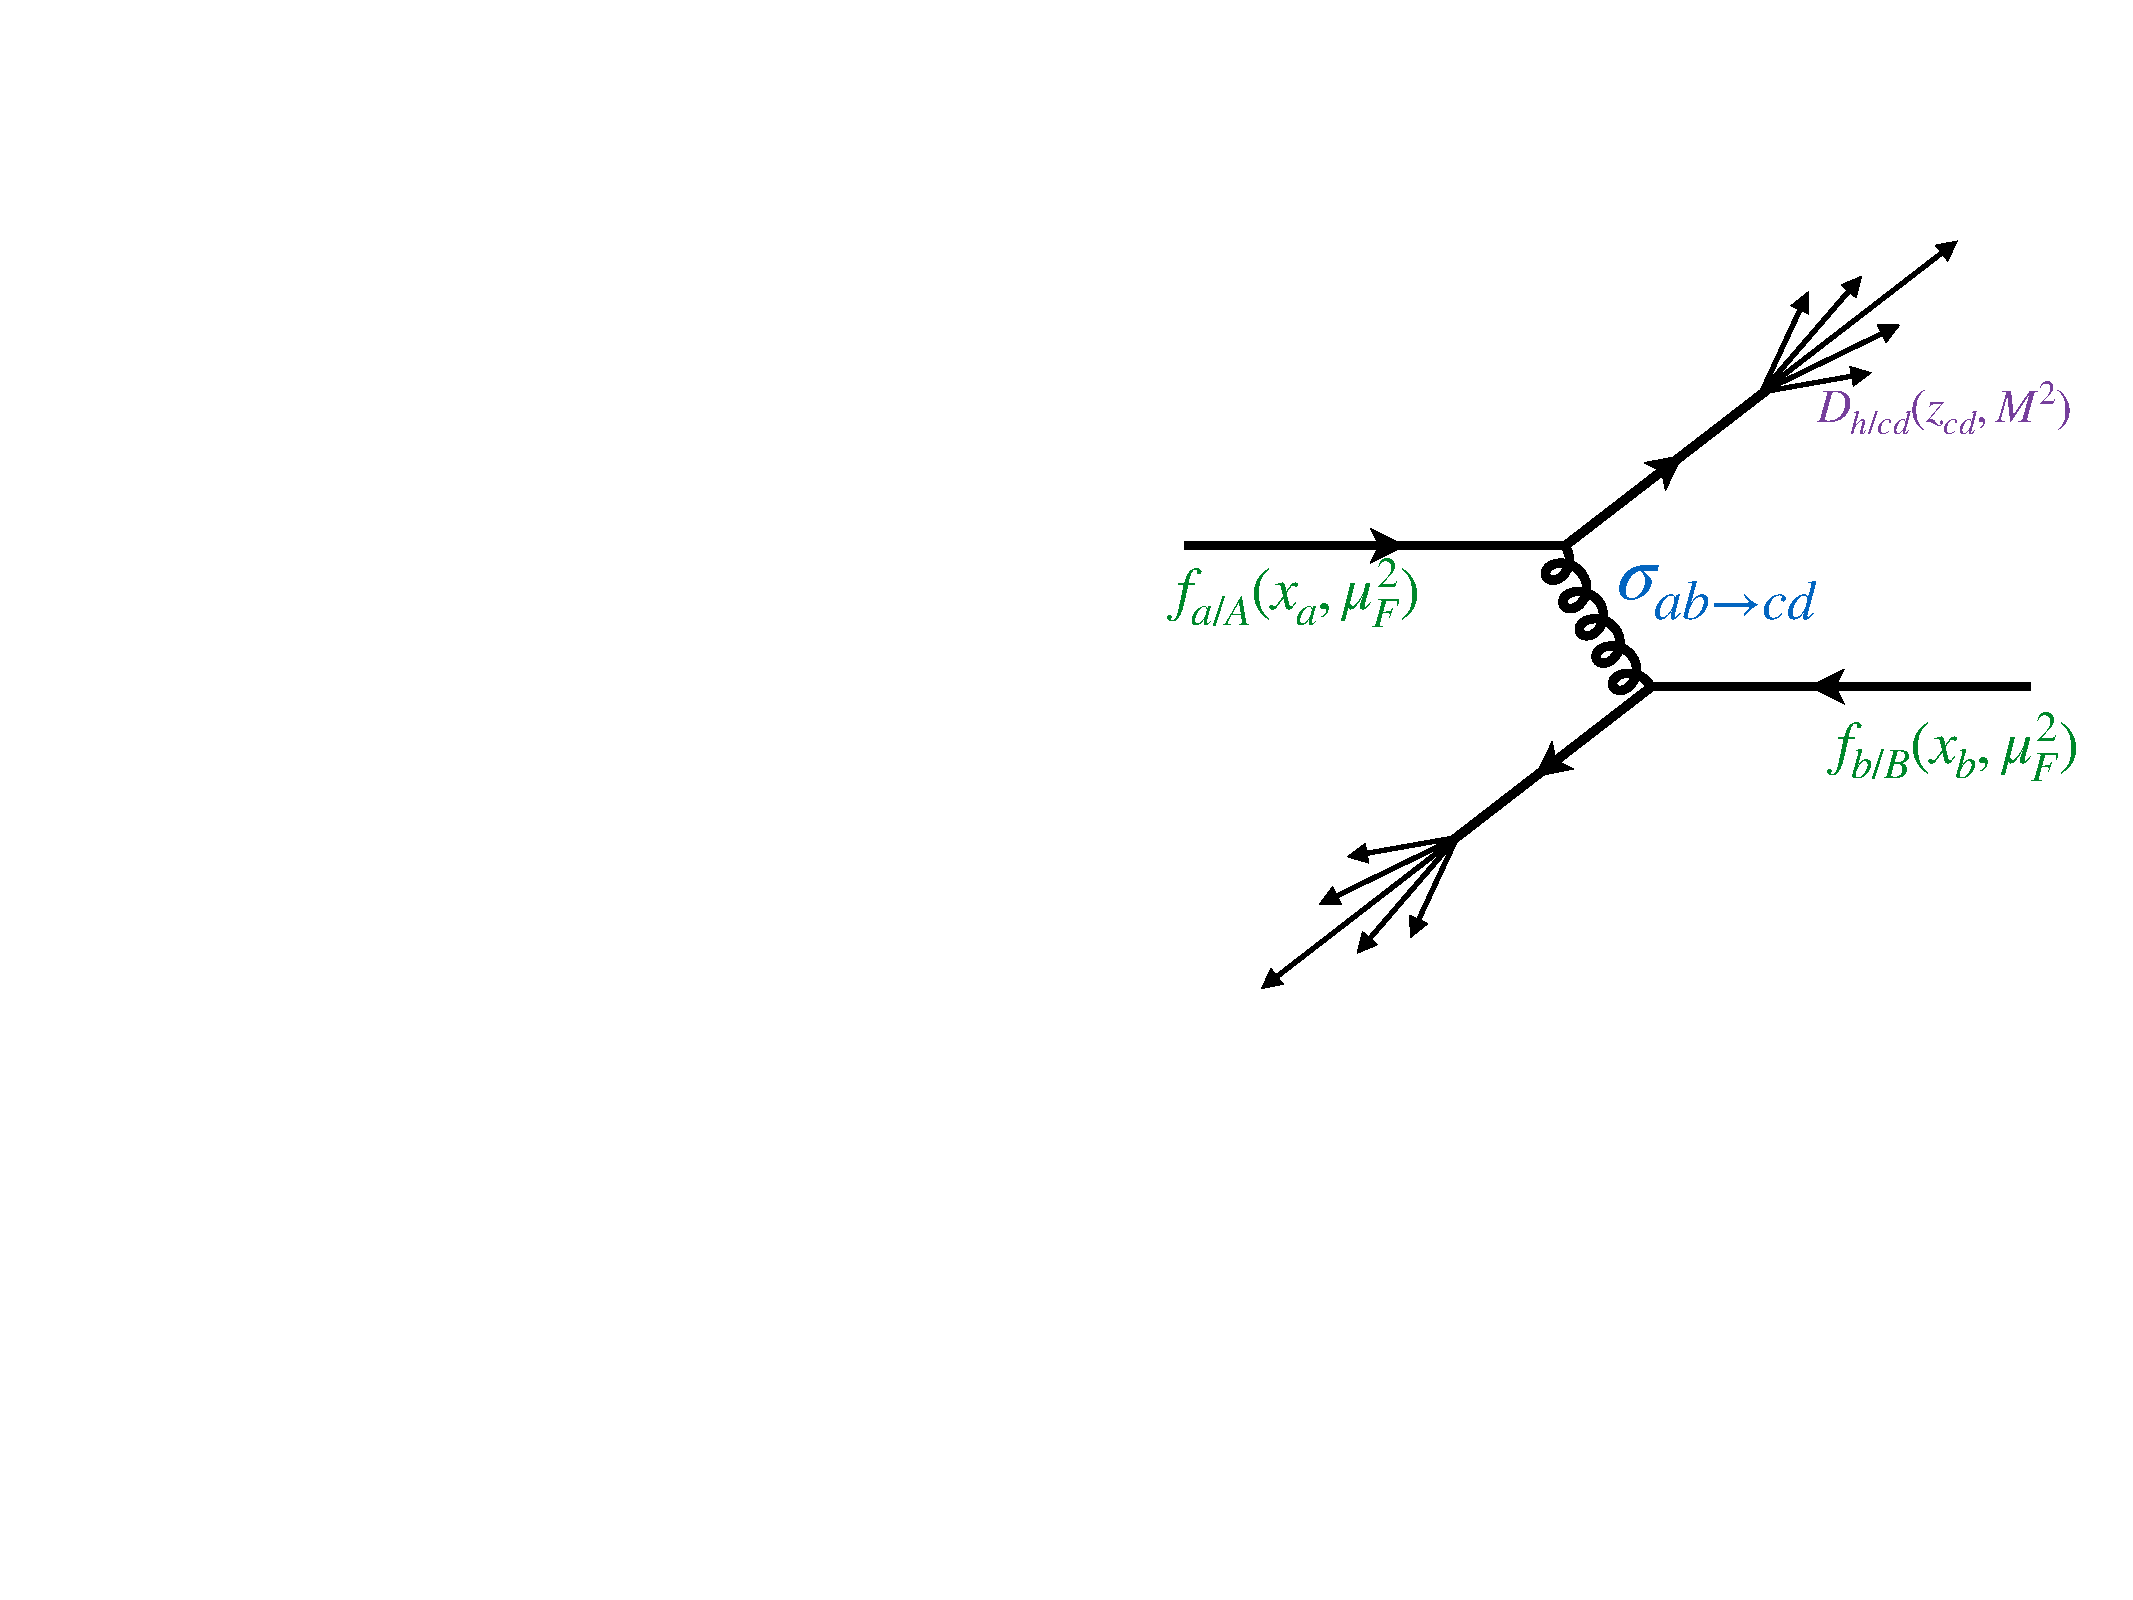
\includegraphics[width=0.35\textwidth]{figures/theory/feynman_jet}
\caption{Jet production from the process $pp \rightarrow hX$, factorizing in terms of the parton distribution functions, scattering cross sections, and jet fragmentation functions. \cite{Qin:2015srf}}
\label{fig:feynman_jet}
\end{center}
\end{figure}



\begin{align}
\label{eq:hadronCS}
d \sigma_{pp \rightarrow hX} \approx & \sum_{abjd} \int dx_a \int dx_b \int dz_j f_{a/p} (x_a, \mu_f) \otimes f_{b/p} (x_b, \mu_f) \\
& \otimes d\sigma_{ab\rightarrow jd} (\mu_f, \mu_F, \mu_R)  \nonumber \\
& \otimes D_{j \rightarrow h} (z_j, \mu_f) \nonumber
\end{align}
where $x_a = p_a/P_A, x_b = p_b / P_b$ are the initial momentum fractions carried by the interacting partons, $z_j = p_h / p_j$ is the momentum fraction carried by the final observed hadron. $f_{a/p} (x_a, \mu_f)$ and $f_{b/p} (x_b, \mu_f)$ are the two parton distribution functions (PDFs), $d\sigma_{ab\rightarrow jd} (\mu_f, \mu_F, \mu_R)$ is the differential cross section for parton scattering and $D_{j\rightarrow }(z_j,\mu_F)$ is the fragmentation function (FFs) for parton $j$ to hadron $h$. $\mu_f$ and $\mu_F$ are the factorization scales and $\mu_R$ is the renormalization scale, and are typically taken to be the same hard scale $Q$. The PDFs characterize the initial state and represent the probability of finding a parton with momentum fraction $x$ (shown in Figure~\ref{fig:bjorkenX}) in the initial hadron, while the FFs describe the probability of fragmenting to a hadron $h$ with given kinematic properties.

\begin{figure}[htbp]
\begin{center}
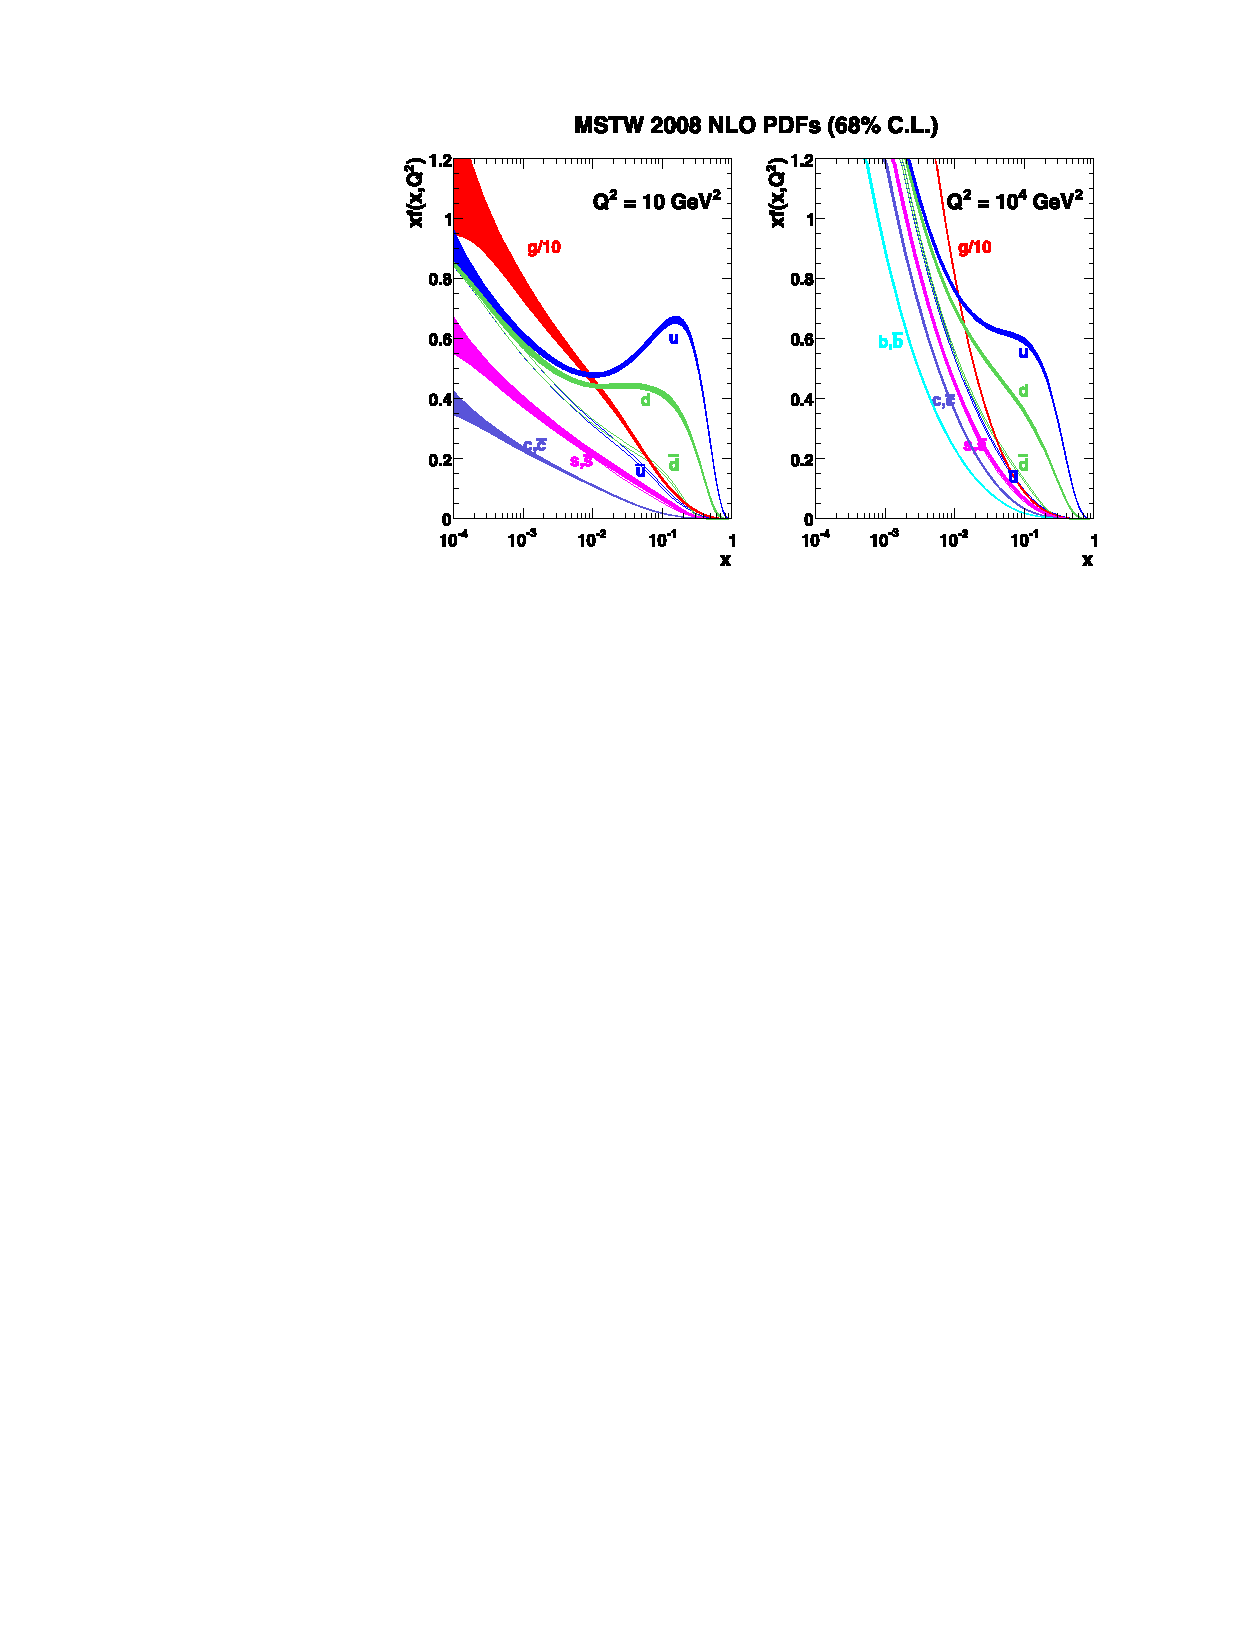
\includegraphics[width=0.55\textwidth]{figures/theory/bjorkenX}
\caption{The next to leading order (NLO) PDFs at (left) $Q^2 = 10 \mathrm{GeV}^2$ and (right) $Q^2 = 10^4 \mathrm{GeV}^2$. The band is the associated one-sigma (68\%) confidence level uncertainty. Taken from \cite{Martin2009}}
\label{fig:bjorkenX}
\end{center}
\end{figure}


%Both the PDFs and FFs are universal and their scale dependence evolves via the Dokshitzer-Gribov-Lipatov-Altarelli-Parisi (DGLAP) equations \cite{ALTARELLI1977298, Gribov:1972ri, Dokshitzer:1977sg}. These calculations can be compared to the inclusive charged particle distributions in \sqrts = 13 TeV \pp\ collisions and shown in Figure~\ref{fig:inclhadronCS}.  



%The energy lost by a jet serves as further confirmation that the medium produced in a heavy ion collision is strongly coupled.

In the case of heavy ion collisions, the jet observables can be modified due to two sources: the nuclear PDF being distinct from a proton PDF, and the formation of the quark gluon plasma.

The former is collectively referred to as cold nuclear matter (CNM) effect, and can be quantified by defining a nuclear modification factor for the PDF:

\begin{align}
R_a^A (x, Q^2) = \frac{f_{a/A} (x, Q^2)}{f_{a/p}(x, Q^2)}
\end{align}
where $f_{a/A}$ and $f_{a/p}$ are the nuclear and proton PDFs respectively. This $R_a^A$ factor is determined by global fits to data from DIS measurements \cite{PhysRevC.76.065207, PhysRevD.69.074028, Eskola_2009}. CNM effects include the following contributions:
\begin{itemize}
\item Shadowing: This is a destructive interference effect that reduces the interactions of a nucleon incident on a nucleus within its interior and on its back face. This effect reduces the effective number of nucleons in an inelastic interaction to $A^{2/3}$. For $Q^2$ of the order of a few $\mathrm{GeV}^2$, this effect dominates for $x < 0.05$ and implies $R_a^A (x, Q^2) < 1$  \cite{PhysRevLett.64.1342}.
\item Anti-shadowing: This compensates for the shadowing effect based on the momentum sum rule, and for $Q^2$ of the order of a few $\mathrm{GeV}^2$ implies $R_a^A (x, Q^2) > 1$ over the region $0.05 < x < 0.20$.
\item EMC: The modification of the nuclear structure function was first observed by the European Muon Collaboration \cite{AUBERT1983275}. Recent observations have suggested that the effect is caused by short-range correlated nucleon pairs within nuclei \cite{PhysRevC.85.047301}. For $Q^2$ of the order of a few $\mathrm{GeV}^2$, this effect dominates for $0.2 < x < 0.80$ and implies $R_a^A (x, Q^2) < 1$.
\item  Fermi Motion: This effect considers the motion of the nucleons within the nucleus. It results in $R_a^A (x, Q^2) > 1$  over the $x > 0.8$ region for $Q^2$ of the order of a few $\mathrm{GeV}^2$ \cite{Saito:1985ct}.

\end{itemize}

%\subparagraph{Shadowing} This is a destructive interference effect that reduces the interactions of a nucleon incident on a nucleus within its interior and on its back face. This effect reduces the effective number of nucleons in an inelastic interaction to $A^{2/3}$. For $Q^2$ of the order of a few $\mathrm{GeV}^2$, this effect dominates for $x < 0.05$ and implies $R_a^A (x, Q^2) < 1$  \cite{PhysRevLett.64.1342}.
%\subparagraph{Anti-shadowing} This compensates for the shadowing effect based on the momentum sum rule, and for $Q^2$ of the order of a few $\mathrm{GeV}^2$ implies $R_a^A (x, Q^2) > 1$ over the region $0.05 < x < 0.20$.
%\subparagraph{EMC} The modification of the nuclear structure function was first observed by the European Muon Collaboration \cite{AUBERT1983275}. Recent observations have suggested that the effect is caused by short-range correlated nucleon pairs within nuclei \cite{PhysRevC.85.047301}. For $Q^2$ of the order of a few $\mathrm{GeV}^2$, this effect dominates for $0.2 < x < 0.80$ and implies $R_a^A (x, Q^2) < 1$.
%\subparagraph{Fermi Motion} This effect considers the motion of the nucleons within the nucleus. It results in $R_a^A (x, Q^2) > 1$  over the $x > 0.8$ region for $Q^2$ of the order of a few $\mathrm{GeV}^2$ \cite{Saito:1985ct}.

Cold nuclear matter effects are experimentally measured using $p+A$ systems where the size and shape of the plasma, and hence any effects thereof, are a lot smaller. 

The second source of modification is the formation of the hot and dense quark gluon plasma. The hot nuclear matter effects further serve as an independent confirmation that the medium formed is strongly interacting. Jets are formed early enough that they traverse the Quark Gluon Plasma and as strongly interacting particles, are both affected by, and affect the QGP. This interaction typically results in the jet losing energy and forward momentum \cite{2012176, ATLAS:2017wvp}, with the lost energy being deposited in the medium \cite{Khachatryan2016}. Jets can also pick up momentum transverse to the parton direction \cite{Chatrchyan:2012nia}. The hot nuclear matter effects can be considered to be a combination of collisional and radiative energy losses summarized in Figure~\ref{fig:jetEnergyLoss}.

\begin{figure}[htbp]
\begin{center}
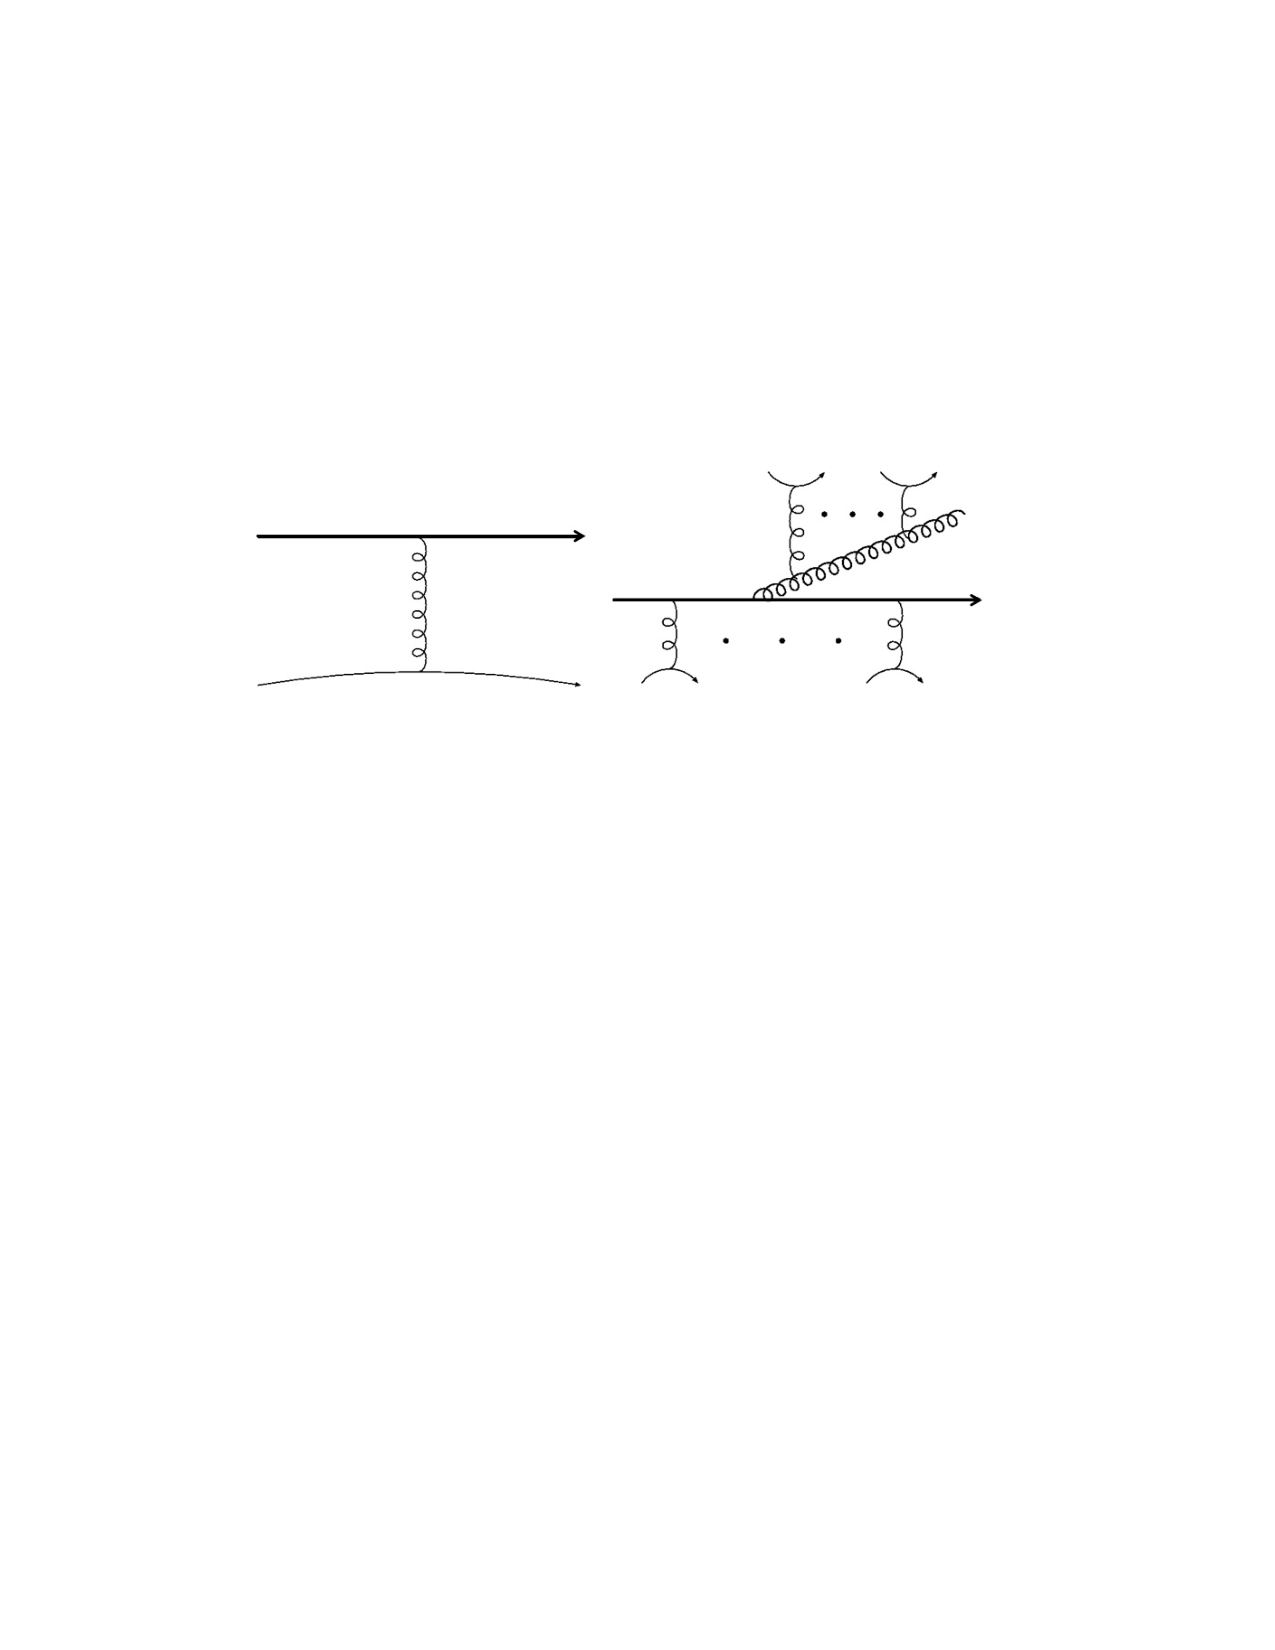
\includegraphics[width=0.75\textwidth]{figures/theory/jetEnergyLoss}
\caption{The typical diagrams for (left) collisional and (right) radiative energy losses for a parton in a hard scattering as it propagates through the QGP. Taken from \cite{Qin:2015srf}}
\label{fig:jetEnergyLoss}
\end{center}
\end{figure}

\begin{itemize}
\item Collisional energy loss: This is a combination of elastic and inelastic collisions of the hard parton with the constituents of the quark gluon plasma. 
\item Radiative energy loss: This is the larger source of parton energy loss and jet quenching. These are modified by the presence of the plasma due to scatterings off of the plasma constituents. A variety of radiative energy loss frameworks that have been developed include: Baier-Dokshitzer-Mueller-Peigne-Schiff-Zakharov (BDMPS-Z) \cite{BAIER1997291}, Gyulassy, Levai and Vitev (GLV) \cite{Gyulassy:1999zd}, Amesto-Salgado-Wiedemann (ASW) \cite{Wiedemann:2000za},  Arnold-Moore-Yaffe (AMY) \cite{Arnold:2001ba} and higher twist (HT) \cite{Guo:2000nz}.
\end{itemize}

\subparagraph{Collisional energy loss} This is a combination of elastic and inelastic collisions of the hard parton with the constituents of the quark gluon plasma. The 

Both hot and cold nuclear matter effects can be described by modifying Equation~\ref{eq:hadronCS} as:
\begin{align}
d \sigma_{AB \rightarrow hX}  \approx & \sum_{abjj'd} f_{a/A} (x_a) \otimes f_{b/B} (x_b) \\ 
& \otimes d\sigma_{ab\rightarrow jd} (\mu_f, \mu_F, \mu_R)  \nonumber \\
& \otimes P_{j\rightarrow j'} \nonumber \\
& \otimes D_{h \rightarrow j'} (z_j, \mu_f) \nonumber 
\end{align}

where the additional $P_{j\rightarrow j'}$ describes the interaction of the hard parton with the colored medium. This is typically taken as part of the fragmentation modification as:

\begin{align}
\widetilde{D}_{h \rightarrow j'} (z_j, \mu_f) \approx \sum_{j'} P_{j\rightarrow j'} (p_{j'} | p_j) \otimes D_{h\rightarrow j'} (_{j'})
\end{align}

A few jet measurements and their modifications by the presence of the Quark Gluon Plasma are discussed in Section~\ref{sec:jetMeasurements}.


%%%%%%%%%%%%%%%%%%%%%%%%%%%%%%%%%%%%%%%%%%%%%%%%
%  jet cross section in  \sqrts = 13 TeV \pp\ collisions can be seen in Figure~\ref{fig:incljetCS}
%
%
%
%\begin{figure}[htbp]
%\begin{center}
%\includegraphics[width=0.55\textwidth]{figures/theory/incljetCS}
%\caption{The inclusive jet cross section as a function of \pt\ and $|y|$ as measured by ATLAS. The data are compared to NLO pQCD calculations. Taken from \cite{Aaboud:2017wsi}}
%\label{fig:incljetCS}
%\end{center}
%\end{figure}
%
%
%
%
%

%
%\begin{figure}[htbp]
%\begin{center}
%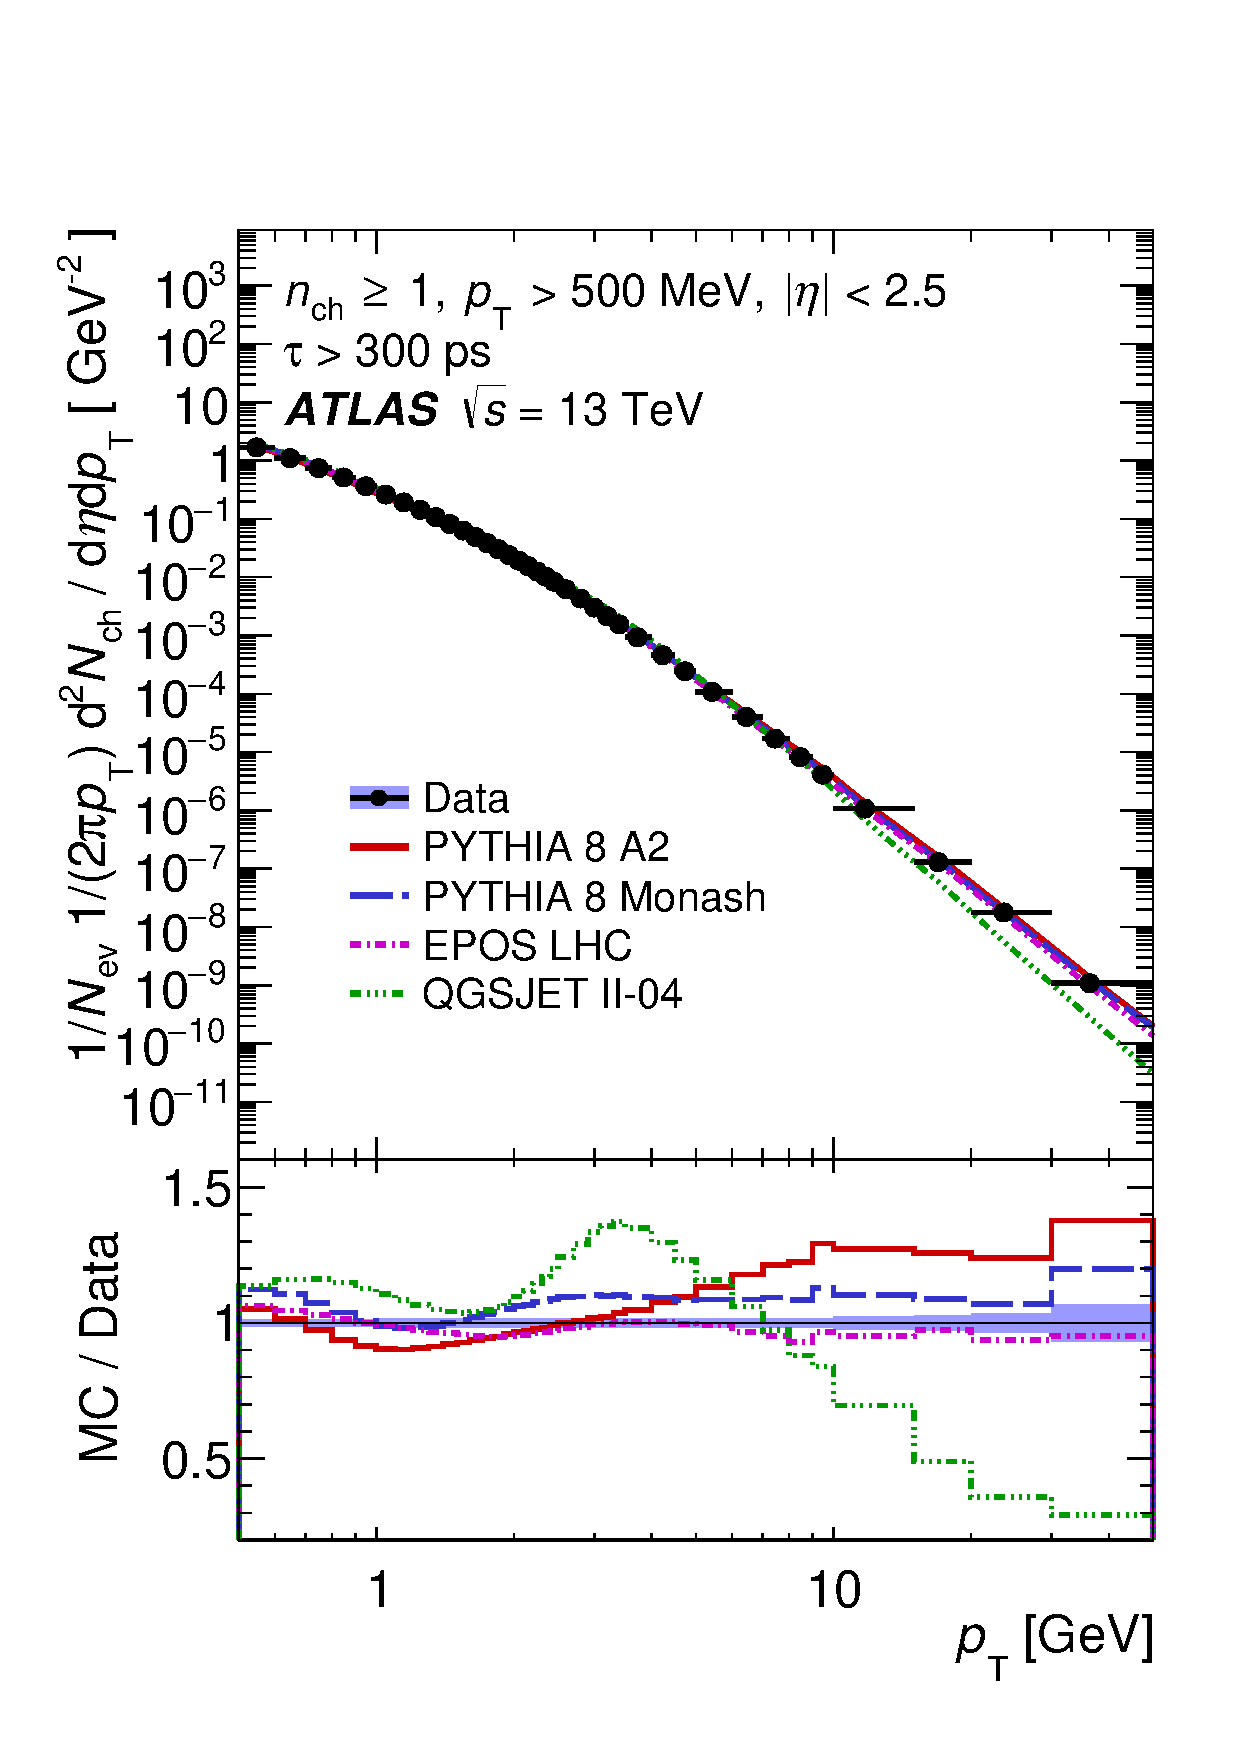
\includegraphics[width=0.55\textwidth]{figures/theory/inclhadronCS}
%\caption{The charged particle multiplicities as a function of transverse momentum \pt\ in \sqrts = 13 TeV \pp\ collisions as measured by ATLAS. The data are compared to NLO pQCD calculations. Taken from \cite{201667}. }
%\label{fig:inclhadronCS}
%\end{center}
%\end{figure}
%
%
%
%Equation~\ref{eq:hadronCS} is written at leading order (LO) and includes contributions from $2\rightarrow2$ cross sections, LO re-summed PDFs and FFs, and single loop expression for the strong coupling \alphas. At next to leading order (NLO), the contributions from real $2\rightarrow3$ and virtual $2\rightarrow3$ processes, as well as the double loop expression for \alphas are included. These calculations describe the inclusive and pQCD, NLO calculations have next to leading order (NLO) calculations that include Figure~\ref{fig:incl_hadron_CS} hows the inclusive jet cross section as measured by ATLAS in \sqrts = 13 TeV \pp\ collisions. 
%
%
%
%
%In a heavy ion collision where the QGP is formed, the hard scattering interactions between the partons strongly interact with the QGP due to their color charge and are modified and lose energy via collisions with the medium constituents, or gluon bremsstrahlung. 